\documentclass[a4paper, 12pt, titlepage]{article}

% Including needed packages
\usepackage[margin=2cm]{geometry}
\usepackage{amsmath}
\usepackage{amssymb}
\usepackage{amsthm}
\usepackage{graphicx}
\usepackage{subfig}
\usepackage{float}
\usepackage{pgf}
\usepackage{tikz}
\usepackage{dsfont}

\newcommand{\norm}[1]{\lVert#1\rVert}
\usetikzlibrary{automata,positioning}

\title
{{\em Machine learning 2}\\
Exercise sheet 10}
\author{FLEISCHMANN Kay, Matrnr: 352247\\
	ROHRMANN Till, Matrnr: 343756}
\date{\today}

\begin{document}

\maketitle
\section*{Hidden Markov Model}

Let $A_{i,j}$ the transition matrix between hidden states $x_i$ and $x_j$. $B_{i,j}$ is the the probability, beeing in state $x_i$ to observe $y_j$.
The following matrices $A$ and $B$ describe two hidden states and two possible observations.

\[
A= 
 \begin{pmatrix}
  0.1 & 0.9 \\
  0.5 & 0.5
 \end{pmatrix}
\]

\[
B=
 \begin{pmatrix}
  0.2 & 0.8 \\
  0.4 & 0.6
 \end{pmatrix}
\]

\subsection*{19.a Implementation of Viterbi algorithm}
\subsection*{19.b Experiment results}

Perform the following experiment: for the Hidden Markov Model of sheet 9, that is, generate sequences of length $l= 5, 10$ and $20;$ for each length generate a number of $N = 1000$ pairs of output sequences and hidden state sequences. On these sequences, for each length , compare $(i)$ the Viterbi algorithm and $(ii)$ the algorithm which randomly uniformly estimates a state sequence by (i) plotting for each length , and all integers $1 \le k \le l$ , the relative frequency of the algorithm correctly estimating the hidden state at position $k$ (this is three plots, one for each , and in each plot two curves), and $(ii)$ for each length , computing the relative frequency of both algorithms succeeding in completely identifying the state sequence correctly (this is two numbers for each of the three). 
The results are given in figure \ref{fig:results}.
The prediction accuracies for the whole hidden state sequences of the different methods is given in the title of the matlab plots and in table \ref{tab:acc}.

\begin{figure}[h]
	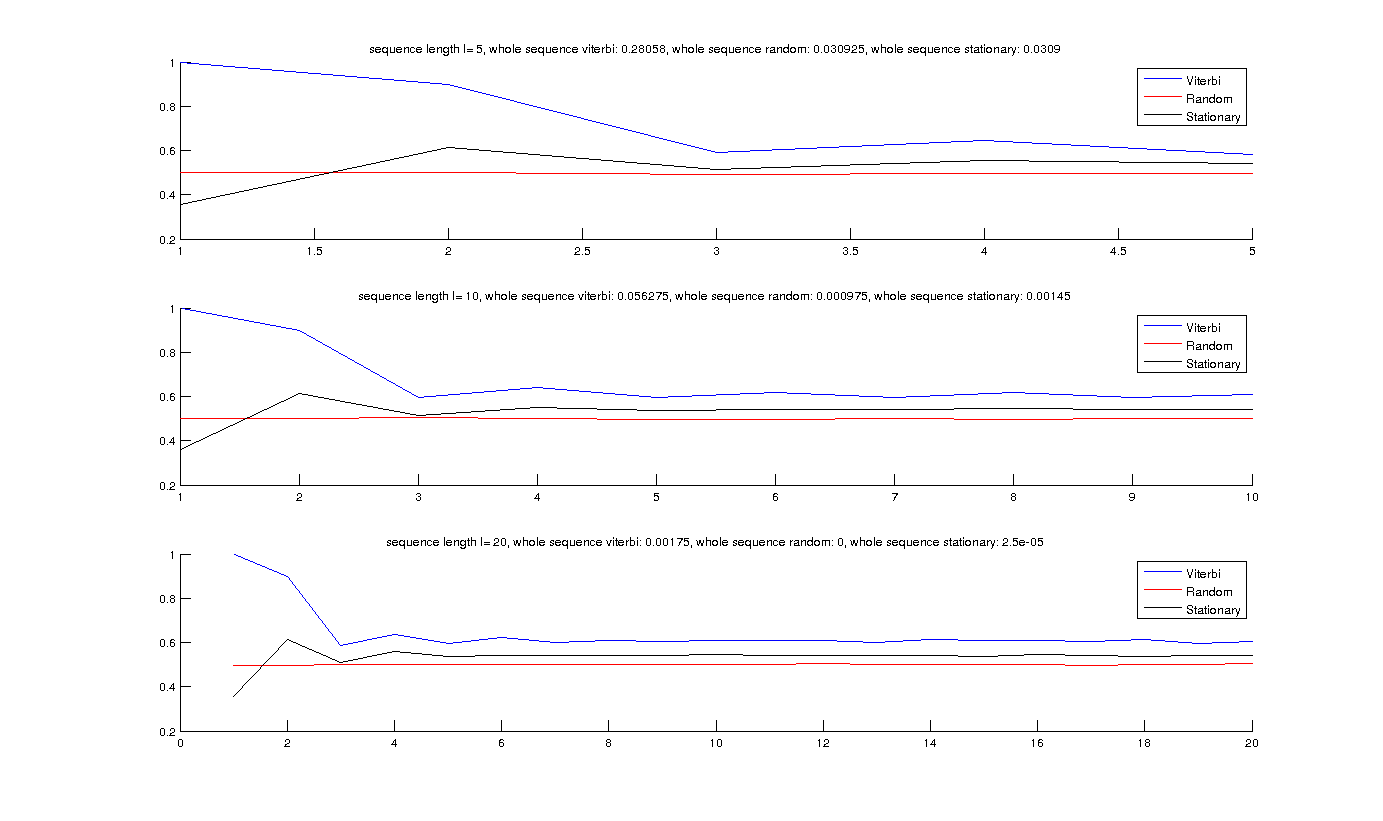
\includegraphics[width=18cm]{images/experiment_results.png}
	\caption{These plots compare the viterbi algorithm results with the uniformly sampled hidden states and the hidden states sampled from the stationary distribution $\pi_{\infty}$. The plots show the relative correct detected hidden states with respect to their positions for different observation lengths. Furthermore, the titles show the prediction accuracy for the whole state sequence.}
	\label{fig:results}
\end{figure}

\begin{table}
	\centering
	\begin{tabular}{llll}
	Method & length $5$ &length $10$ & length $20$\\
	\hline
	viterbi & $0.28058$ & $0.030925$ & $0.0309$\\
	uniformly & $0.056275$ & $0.000975$ & $0.00145$\\
	stationary & $0.00175$ & $0$ & $0.000025$
	
	\end{tabular}
	\caption{Prediction accuracies of the whole hidden state sequence of the different methods}
	\label{tab:acc}
\end{table}

\section*{c}

Prove that the limit $\pi_\infty = \lim_{k\rightarrow \infty} \pi \cdot A^k$ exists and that it does not depend on the choice of $\pi$.

\begin{proof}
First we have to prove that the limit exists.
This can be achieved by showing that the matrix multiplication of two stochastic matrices has a stochastic matrix as the result.
Let $A$ and $B$ be two square stochastic matrices.
Then the product is $C = A \cdot B$.
Since $A$ and $B$ were positive, $C$ has to be positive as well.
Let us now check the row sums.
\begin{eqnarray*}
	\sum_{j=1}^N c_{i,j} &=& \sum_{j=1}^N \sum_{k=1}^N a_{i,k}\cdot b_{k,j}\\
	&=& \sum_{k=1}^N a_{i,k} \underbrace{\sum_{j=1}^N b_{k,j}}_{=1}\\
	&=& \sum_{k=1}^N a_{i,k}\\
	&=& 1
\end{eqnarray*}

Thus for any $k$, $A^k$ is well defined and has a finite norm.
Consequently, the limit $\lim_{k\rightarrow \infty} \pi \cdot A^k$ exists.

Now we have to show that the limit $\pi_{\infty}$ is reached for any initial distribution $\pi$.
This is the case, if the limit $\lim_{k\rightarrow \infty} A^k$ is a matrix such that each column contains in each row the same value.
In the case of our $A$, this could be
\begin{eqnarray*}
	\lim_{k\rightarrow \infty} A^k &\approx& \begin{pmatrix}
  0.3571 & 0.6429 \\
  0.3571 & 0.6429
 \end{pmatrix}
\end{eqnarray*}

There we can see that for any $\pi$ $\pi_{infty} = (0.3571,0.6429)$.
Furthermore, let us assume that we can represent each column as a linear combination of orthogonal eigenvectors, this means each column 
\begin{eqnarray*}
	a_j &=& \sum_{i=1}^N c_i\cdot v_i
\end{eqnarray*}

with $v_i$ being the eigenvectors and $c_i$ the coefficients.
Then the operation $A\cdot A$ has the following consequence on the columns:
\begin{eqnarray*}
	a_j^2 &=& \sum_{i=1}^N \lambda_i \cdot c_i \cdot v_i
\end{eqnarray*}

And the columns of $A^k$ would be
\begin{eqnarray*}
	a_j^k &=& \sum_{i=1}^N \lambda_i^{k-1} \cdot c_i \cdot v_i
\end{eqnarray*}

Thus all eigenvectors with eigenvalues with a real part smaller than $1$ will vanish and only those with a eigenvalue (again the real part) greater or equal to $1$ will stay.
In fact, we can already conclude that there cannot be any eigenvalues greater than $1$, because otherwise the limit $\lim_{k\rightarrow \infty} A^k$ would not exist.

For the sake of completeness, here the derivation:
Let $v$ be an eigenvector with eigenvalue $\lambda \in \mathds{C}$ of $A$.
Then it holds that $A\cdot v=\lambda \cdot v$.
Let $i=argmax_{j} |v_{j}|$ be the component of $v$ with maximum absolute value.
\begin{eqnarray*}
	|\lambda| |v_{i}| &=&| \sum_{j} a_{i,j} v_{j} |\\
	&\le& \sum_{j} |a_{i,j}||v_{j}| \\
	&\le& \sum_{j} a_{i,j} \max_{k}(|v_{k}|)\\
	&=& |v_{i}| \sum_{j} a_{i,j}\\
	&=& |v_{i}|
\end{eqnarray*}

Thus the absolute value of all eigenvalues is smaller or equal to $1$.
We can now observe that the vector $\mathds{1}$ is an eigenvector of $A$ with $\lambda=1$ as its eigenvalue because $A \cdot \mathds{1} = \mathds{1}$.
If this were the only eigenvector for the eigenvalue $1$, we could finish the proof, because then each column of $A^k$ would converge against the eigenvector $\mathds{1}$ multiplied by a scalar coefficient and this is what we had to show.
Luckily, the Perron-Frobenius theorem gives us exactly this.
It says for positive square matrices that the eigenvalue with maximum absolute value is a simple eigenvalue.
Consequently, $\mathds{1}$ can be the only eigenvector with eigenvalue $\lambda=1$ and all other eigenvectors will vanish.
Since the scalar products of the columns of $A$ with $\mathds{1}$ are non-zero and positive, the eigenvector $\mathds{1}$ is contained in all linear combinations.
Therefore, all columns of $A$ will converge against a positive multiple of $\mathds{1}$.

\end{proof}

\section*{d}

Instead of uniformly sampling the state sequence we used the stationary distribution $\pi_{\infty} = (0.3571,0.6429)$ to sample our state sequnce. The results can be seen in figure \ref{fig:results}
We can clearly see that the sampling with the stationary distribution produces a higher prediction correctness for the individual states at the different positions.
However, the whole sequences are only better predicted for long state sequences where the markov chain has reached its stationary distribution.

\end{document}
